\subsection{Determine reference yaw rate for ESC}

The steady state yaw rate gain for the bicycle model is expressed as the following:

\begin{equation}
    \frac{\omega}{\delta_f} = \frac{v_x}{L + K_u m v_x^2}
\end{equation}

This can be used to calculate reference yaw rate for a given vehicle speed $v_x$ and steering angle $\delta_f$. This reference is expressed as the following:

\begin{equation*}
    \omega_{ref,1} = \frac{v_x \delta_f}{L+K_u m v^2}
\end{equation*}

However, this does not take into account the maximum lateral force that the tyres can provide. This means that during the beginning of the maneuver, with a high steering angle $\delta_f$, the reference $\omega_{ref,1}$ is going too be to high. This could cause the system to induce oversteer as to increase the yaw rate, which would make the vehicle unstable during the beginning of the maneuver. 

Another limit is therefore needed to account for the maximum lateral force that the tyres can provide. Assuming that the maximum lateral force $Fy$ is provided. 

\begin{align*}
    \sum Fy = \sum F_z \mu_{0} & = \mu_0 mg = m a_y \Rightarrow  \\
    & a_{y,max} = \mu_0 g
\end{align*}

This can the be use to calculate the maximum available yaw rate as:

\begin{equation*}
    \omega_{ref,2} = \frac{a_{y,max}}{v_x} = \frac{\mu_0 g}{v_x} 
\end{equation*}

The final yaw rate reference $\omega_{ref}$ is then expressed as the signed minimum of these two. In matlab this was expressed as:

\begin{equation*}
    \omega_{ref} = sign(\omega_{ref,1})*min(|\omega_{ref,1}|,\omega_{ref,2})
\end{equation*}

This was evaluated in the upcoming questions, where $\omega_{ref}$ is plotted against the actual yaw rate. 

\subsection{Add the control algorithm for the ESC system}
In order to induce an oversteer or understeer, the ESC will brake on of the tires to create a moment around the center of gravity.
During a turn, if a car is oversteering, one of the outer wheels is braked. However, during an understeering situation, one of the inner wheels is braked by the ESC. To know which wheel to brake, front or rear, one has to look at the direction of the force and check which force has a longer moment arm.

\begin{figure}[H]
    \centering
    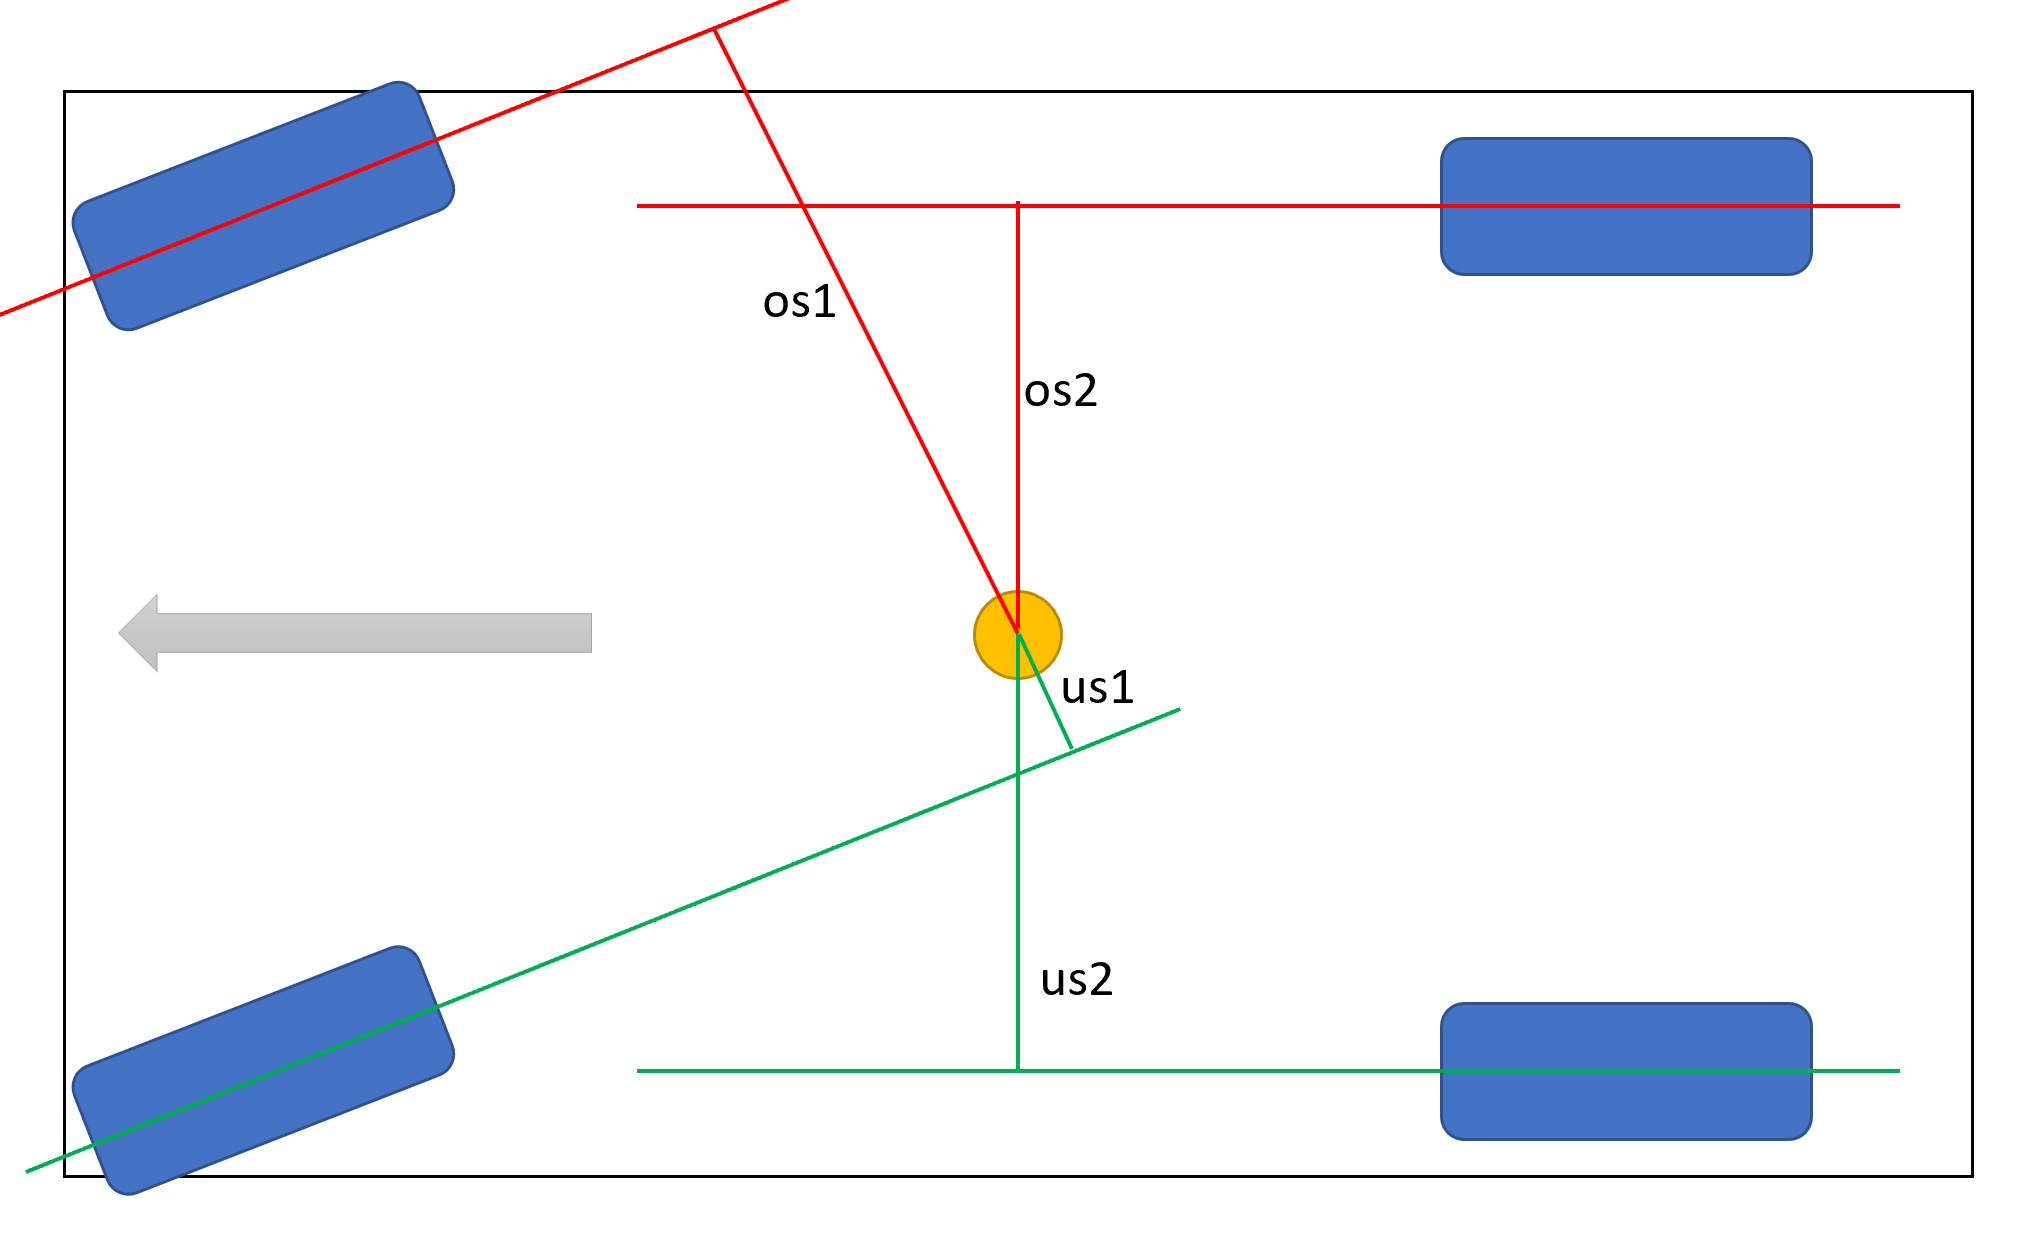
\includegraphics[width=0.7\textwidth]{Figures/underover.PNG}
    \caption{ESC Design Strategy}
    % \label{fig:my_label}
\end{figure}

By looking at the figure above, during oversteer, braking the front outer tire has a bigger moment arm compared to the rear wheel. This is the opposite for the understeer case where the moment arm of the force on the rear wheel is bigger than that on the front.

Hence the design is as follows:
\begin{itemize}
    \item Understeer: Brake inner rear wheel
    \item Oversteer: Brake outer front wheel
\end{itemize}

In Matlab, this algorithem was implemented as such, where $\omega =r$:

\begin{lstlisting}
 rErr = abs(r-rREF);

     FxReq = [0; 0; 0; 0;];
    if rErr > rErrLim && vx > uESCLim
        if abs(rREF) > abs(r)           % understeer
            if rREF > 0                 % left turn
                FxReq(3) = -escK*rErr;
            else                        % right turn
                FxReq(4) = -escK*rErr;
            end
        else                            % oversteer
            if rREF > 0                 % left turn
                FxReq(2) = -escK*rErr;
            else                        % right turn
                FxReq(1) = -escK*rErr;
            end
        end
    end
\end{lstlisting}

\subsection{Evaluate ESC performance and check side slip angle}

With the ESC enabled, the vehicle passed all the tests in the given region SWD $\in[60,300]\degree$. As to evaluate how it changes the vehicle's handling, a simulation was run with a steering angle of $140\degree$, since this is comparable with the base case. 

\begin{figure}[H]
      \begin{minipage}[b]{0.5\linewidth}
      \centering
        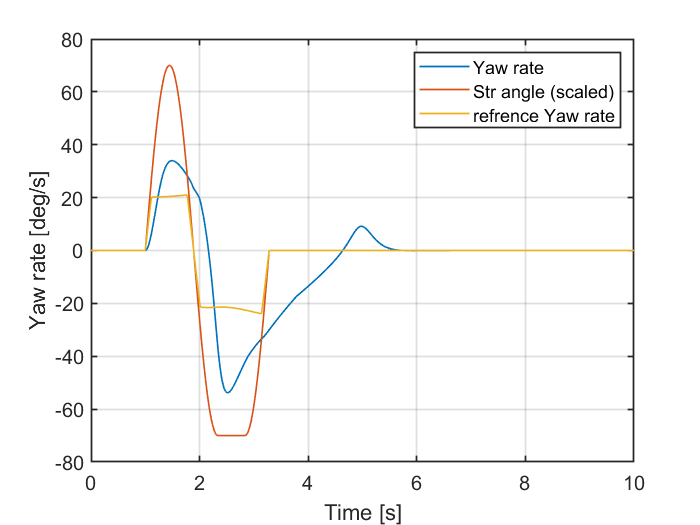
\includegraphics[width=\linewidth]{Figures/3_3_ESCon.png}
        %  \caption*{Trajectory} 
        % \label{fig:2_4_l}
    \end{minipage} 
    \begin{minipage}[b]{0.5\linewidth}
    \centering
        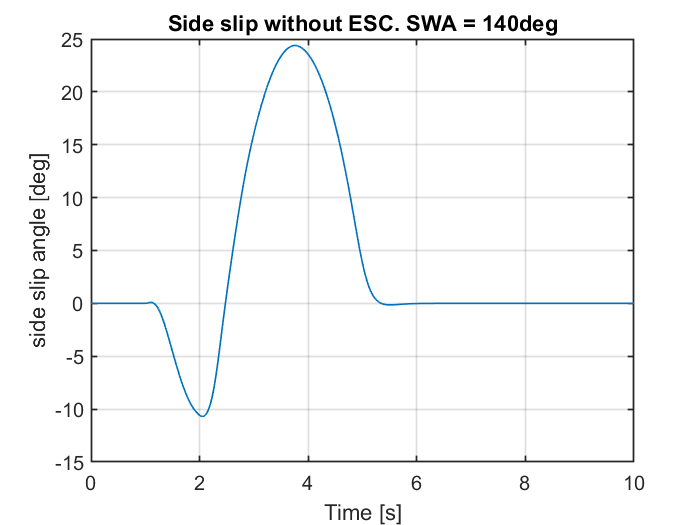
\includegraphics[width=\linewidth]{Figures/3_3_ESCon_sideSlip.png}
        % \caption{Yaw rate}
        % \label{fig:2_4_u}
    \end{minipage} 
    \caption{Side Slip and Yaw Rate with Load Transfer for Sine with Dwell Test with SWA 140\degree}
    %  \label{fig:headbodyrelmotion}
\end{figure}

As apparent by the figure above, side slip angle is lower than the case with ESC off and the yaw rate stabilises faster. This means that the vehicle is overall more stable and more responsive to steering input, even in transient motions. This would make the driver feel that the vehicle is more stable with ESC on, which is desirable.  

